\chapter{Probabilistic Variational Model}
\label{chap:statistical_model}

\lettrine{G}{ranting} a system an accommodative behavior beyond a direct response to the user's input is a major and understudied challenge in \acs{hci}.
In live \acsp{hhi}, the behavior of a speaker varies both within and across conversations.
This chapter presents a statistical approach that generates variational behaviors, which can be integrated into a \acl{sds} to offer non-deterministic accommodative outputs.

\pagebreak

\acresetall

\noindent
The statistical approach presented in this chapter offers a different way to model and simulate accommodative behaviors.
It determines the system's next output value based on probabilities calculated from a dataset, unlike the method introduced in \cref{chap:computational_model} where the output value is determined based on pre-defined parameters.
While the latter achieves \emph{responsiveness} in a \ac{sds} per the definition in \cref{subsec:accommodation_levels}, the former grants \emph{profiles} and \emph{variability}.
This is done using two ways to describe accommodation in a conversation.
The first is a continuous representation, where the speakers' productions are treated as time series and interpolated.
The chosen interpolation lines estimates the speakers' productions for the whole conversation, as explained in \cref{sec:time_series_analysis}.
The second representation uses accommodation categories to describe the nature of the mutual changes observed in the speakers' productions (e.g., convergence or divergence).
As shown in \cref{sec:accommodation_as_a_lm}, these categories allow to represent accommodation more abstractly and give meaning to the productions' raw values.
Using this unified representations, n-gram probabilities of these categories can be calculated to predict the next accommodation event in a conversation.
\Cref{sec:clustering_and_incremental_generation} shows how these two representations are combined into one statistical model.
The overall type of change is generated by the n-gram probabilities and the specific variational value is determined by selecting an interpolation line based on the already observed productions.
This process is demonstrated by clustering speaker behaviors from a dataset to generate different system outputs for a given user input.

\section{Time series representation with \aclp{gp}}
\label{sec:time_series_analysis}

The approach presented in this chapter capitalizes on the temporal nature of spoken interaction, with emphasis on the evolution of mutual accommodation over the course of an interaction, which expands upon the temporal analyses performed in \cref{chap:conv_analysis,chap:speech_variations_in_hhci}.
As in those chapters, features' values are chronologically sampled across equal time intervals, and are therefore treated as \emph{time series}.
%Time series are used for both analysis and prediction in many fields, like anomaly detection, econometrics, seismology, geophysics, and more.
By extension, accommodation can be viewed as time series ass well.
This is motivated by the arguments explained in \cref{subsec:temporal_analysis}, vis.\ that representing mutual changes by merely a few points throughout an interaction or directly comparing its beginning state to its end state is not very informative and draws a rather simplistic picture (see \cref{subsec:limitations_of_did} and \cref{fig:accommodation_types} for details and examples).

This variability in this approach is achieved by fitting a \emph{\ac{gp}} to each speaker.
\Acp{gp} are stochastic processes with a multivariate normal distribution for each random variable.
A \ac{gp} provides the joint distribution for infinitely many random variables, i.e., a \emph{distribution over functions} that match the given evidence.
Specifically, \acp{gp} are used here for \emph{kriging} (\cref{subsec:interploating_data_using_kriging}), an interpolation technique used for time series interpolation and prediction.
The utilization of \acp{gp} provides not only continuous likelihood line for the observed features, but also an infinite number of non-deterministic alternatives -- the variations -- to generate vocal behaviors by randomly sampling from a \ac{gp}.
The generation process presented here can be combined with the aforementioned computational model to harness the benefits of both, as discussed in \cref{subsec:comb_comp_stat_models}.

\subsection{Kernel building and tuning}
\label{subsec:covariance_functions}

\begin{figure}[t]
	\centering
	\subfigure[RBF kernel prior ($length scale = 1$)]
		{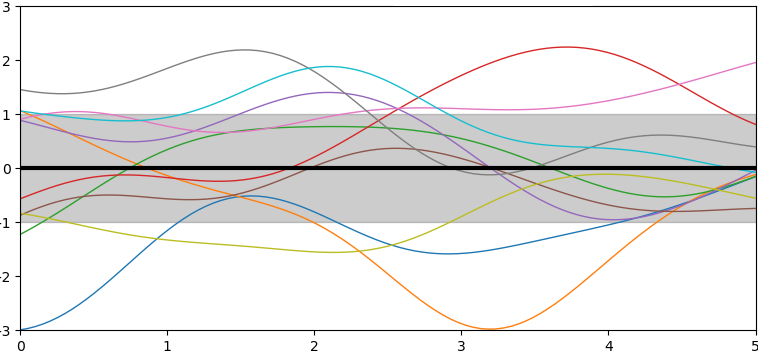
\includegraphics[width=0.45\textwidth]{RBF_prior}
	\label{fig:RBF_prior}}
	\hfill % no empty line here to avoid staring a new paragraph (figures will be vertically aligned)
	\subfigure[RBF kernel posterior ($length scale = 0.279$)]
		{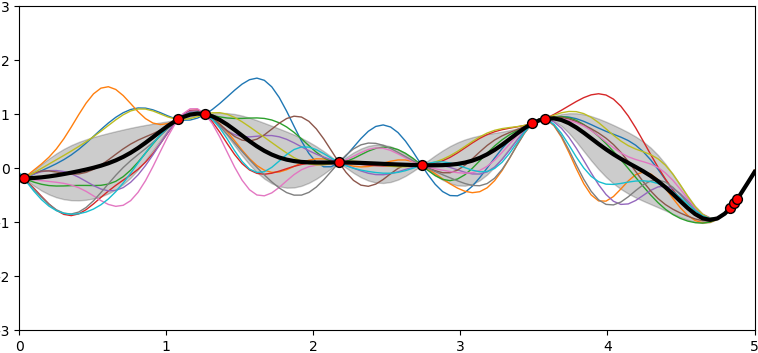
\includegraphics[width=0.45\textwidth]{RBF_posterior}
	\label{fig:RBF_posterior}}
	\caption[Prior and posterior of an RBF kernel]
		{\hspace{-0.18cm}\footnotemark\ 
		Prior and posterior distributions of an RBF kernel with mean zero, resulted in a Gaussian process $\mathcal{GP}\left( 0 (\vec{x}), \Sigma(\vec{x}) \right)$.
		Each color line stands for a drawing (prediction) from the prior and posterior distributions, and the thicker black line shows the overall mean of the distributions.
		The red circles are the known datapoints on which the kernel was optimized to fit, and the gray areas mark the \SI{95}{\percent} confidence intervals above and below the overall mean.
		The length scale parameter (in parentheses) determines the length of the \enquote{wiggles} of the functions}
	\label{fig:RBF_prior_posterior}
\end{figure}
\footnotetext{Adapted from \url{https://scikit-learn.org/stable/_images/sphx_glr_plot_gpr_prior_posterior_001.png}}

% \url{http://scikit-learn.org/stable/modules/gaussian_process.html}

Kernels (or \textit{covariance functions}) are a key component in \acp{gp}, as they define the similarity between the \acs{gp}'s random variables.
They define the the covariance $k(x, x')$ between each pair of observed values $x$ and $x'$, so that $k(\cdot, \cdot)$ determines how similar the outputs $y_*$ and $y_*'$ will be.
Formally, a covariance function can be described as $\mathcal{K}(u, v) = \phi(u) \cdot \phi(v)$, where $\phi(\cdot)$ is a function that maps the input vectors into a transformed feature space.
Which function to use is a key consideration when using \acp{gp}, as it determines the behavior of the sampled functions and the nature of the predictions it will be making.
%Naturally, some assumptions and decisions regarding the data must be made when choosing a kernel.
A kernel's parameters are optimized to achieve functions that better fit the data.
Since accommodation analyses deals with the \textit{difference} between production values (as opposed to the values themselves), stationary kernels are more suitable for fitting \ac{gp} for them, as they are shaped by the distances between each pair of datapoints rather than their absolute values.
%That is, they fulfill $k(x_1, x_2) = k(x_1 - x_2)$.
%This list only covers a small subset of common covariance functions.
%Further kernels include the exp-sine squared, dot-product, linear, and more.
A kernel may also be composed of multiple other kernels, to capture a combination of characteristics.
This is done either by multiplication or addition of these kernels.
Multiplication-based kernels are maximized when all of its kernel factors yield high values, whereas
addition-based kernels are maximized when any of their addend kernels yield a high value.
%For example, multiplying a linear kernel by a periodic one will result in functions that are \textit{both} periodic \textit{and} with increasing amplitude as they move away from the origin.
An additive kernel with constant, radial basis function (RBF), and noise terms is used here (see \crefrange{eq:constant_kernel}{eq:RBF_kernel} below).
The RBF term determines the general shape of the curve (see example in \cref{fig:RBF_prior_posterior}), the constant term enables shifting of the curve if necessary, and the noise term adds degrees of freedom in case the curve cannot completely fit the input signal.

The definitions of the individual kernels are as follows:

\begin{description}
	\item[Constant kernel -- ]
	is a simple kernel that assigns the same value for all input pairs.
	Since by itself it does not offer a lot of characteristic to the covariance function, it is usually used in combination with other kernels, where it scales the magnitude of the other factors, or as part of a sum kernel, in which it modifies the mean of the Gaussian process.
	It has a single parameter, the constant value, and it is defined as 
	%
	\begin{equation}
		\label{eq:constant_kernel}
		k_{constant}(\{C\}, x_1, x_2) = C\forall x_1, x_2,
	\end{equation}
	\eqname{Constant kernel}
	%
	where $C$ is the constant value parameter.
	
	\item[Noise kernel -- ]
	is a kernel used for capturing unexplained variation in the data.
	It is typically based on the constant kernel as part of a sum kernel, in which it explains the noise component of a signal.
	In this context, the constant parameter is tuned to estimate the noise level in the interlocutor's mutual change (including distortions caused recognition errors).
	This is determined by
	%
	\begin{equation}
		\label{eq:noise_kernel}
		k_{noise}(\{noise\_level\}, x_1, x_2) =
		\begin{cases}
		C_{noise\_level}, & if\quad x_1 = x_2\\
		0, & otherwise,\\
		\end{cases}
	\end{equation}
	\eqname{Noise kernel}
	%
	where $noise\_level$ equals to the variance of the noise found in the input signal.
	
	\item[Radial-basis function (RBF) kernel --]
	also known as \emph{squared exponential kernel}, this kernel is a stationary kernel with one parameter, \emph{lengthscale} $\ell > 0$.
%	which can either be a scalar (isotropic variant of the kernel) or a vector with the same number of dimensions as the inputs x (anisotropic variant of the kernel).
	This kernel typically results in generally smoothed functions, with the lengthscale being associated with the long-term smoothness and degree of variability on the time dimension.
	The RBF kernel is defined as
	%
	\begin{equation}
		\label{eq:RBF_kernel}
		k_{RBF}(\{\ell\}, x, x') = \sigma^2 exp\left(\frac{\lVert x_1 - x_2 \lVert ^2_d}{2\ell^2}\right),
	\end{equation}
	\eqname{Radial basis function (squared exponential) kernel}
	%
	where $\lVert x_1 - x_2 \lVert$ is the Euclidean distance between two $d$-dimensional input points and $\sigma^2$ is the data variance.
	\cref{fig:RBF_prior_posterior} shows prior and posterior examples of the RBF kernel.
	
%	\item[Rational quadratic kernel]
%	This kernel can be seen as a scale mixture (infinite sum) of RBF kernels with different length scales.
%	Therefore, \acp{gp} priors with this kernel expect to see functions which vary smoothly across many length scales.
%	It has two parameters: length scale $l > 0$ and scale mixture $\alpha > 0$.
%	The parameter $\alpha$ determines the relative weighting of large-scale and small-scale variations.
%	When $\alpha$ $\lim$ $\inf$, the RQ kernel is identical to the SE kernel, as described by
%	
%	\begin{equation}
%		\label{eq:RQ_kernel}
%		k_{RQ}(\{\sigma, \alpha, \ell\}, x, x') = \sigma^2 \left( 1 + \frac{\lVert x_1 - x_2 \lVert ^2}{2\alpha \ell^2} \right)^{-\alpha}.
%	\end{equation}
%	\eqname{Rational quadratic kernel}
\end{description}

\subsection[Data interpolation using kriging]{Data interpolation}
\label{subsec:interploating_data_using_kriging}

As also motivated in \cref{subsec:limitations_of_did,subsec:temporal_analysis}, artificially splitting interactions into a fixed, pre-determined number of parts to measure accommodation results in a limited view on the accommodation events due to sparsity of observation.
To overcome that, the mutual changes should be evaluated continuously throughout the interaction instead of by point-to-point comparisons, where the temporal gaps between datapoints might be greatly unbalanced.
This requires some interpolation method to achieve more general trends based on the observed productions.
One way of achieving that is using some smoothing algorithms, like \ac{loess} in \cref{fig:hds_dds_time}, which is adequate for gaining a smooth estimation of a speaker's overall performance.
A similar approach is used in \citet{Galvez2020unifiying}, in which the average values obtained by \acl{tama} \citep[\acs{tama};][]{Kousidis2008towards, Kousidis2009monitoring} define the behaviors.
However, \ac{tama} values may conceal turns with substantial changes introduced by one of the speakers.
A more evolved approach is presented here to describe a speaker's vocal behavior in a conversation as a distribution over functions that match the accumulated \textit{evidence} from that speaker's productions.

Kriging (or \textit{\acl{gp} regression}) is an interpolation method that gives an optimally fitted and unbiased prediction of intermediate values.
Since this method fits a function distribution over the data, it not only yields mathematically more likely values, but also provides a curve that describes the characteristics of the interpolated curved, as opposed to more naive methods like linear interpolation or smoothing spline.
Another advantage of this method is that it offers a \textit{distribution over functions} rather than specific values.
Therefore, an infinite number of suitable functions can be sampled from one fitted kernel and their likelihood can be evaluated.
Such samples are illustrated in \cref{fig:RBF_posterior}, where each line represents a mean regression prediction drawn from the posterior distribution based on the given datapoints.
This method was applied to each interlocutor in the \ac{hci} portion of the dataset presented in \cref{sec:vacc}.
It is described by
%
\begin{equation}
	\label{eq:gp_function_prediction}
	f_*(\vec{x}) = \mathcal{GP}(\mu_{\vec{x}}, \Sigma_*),
\end{equation}
\eqname{Function predicted using a fitted Gaussian process}\noindent
%
\begin{figure}[t]
	% 20171121A_Calendar_01 was used for the plot
	\centering
	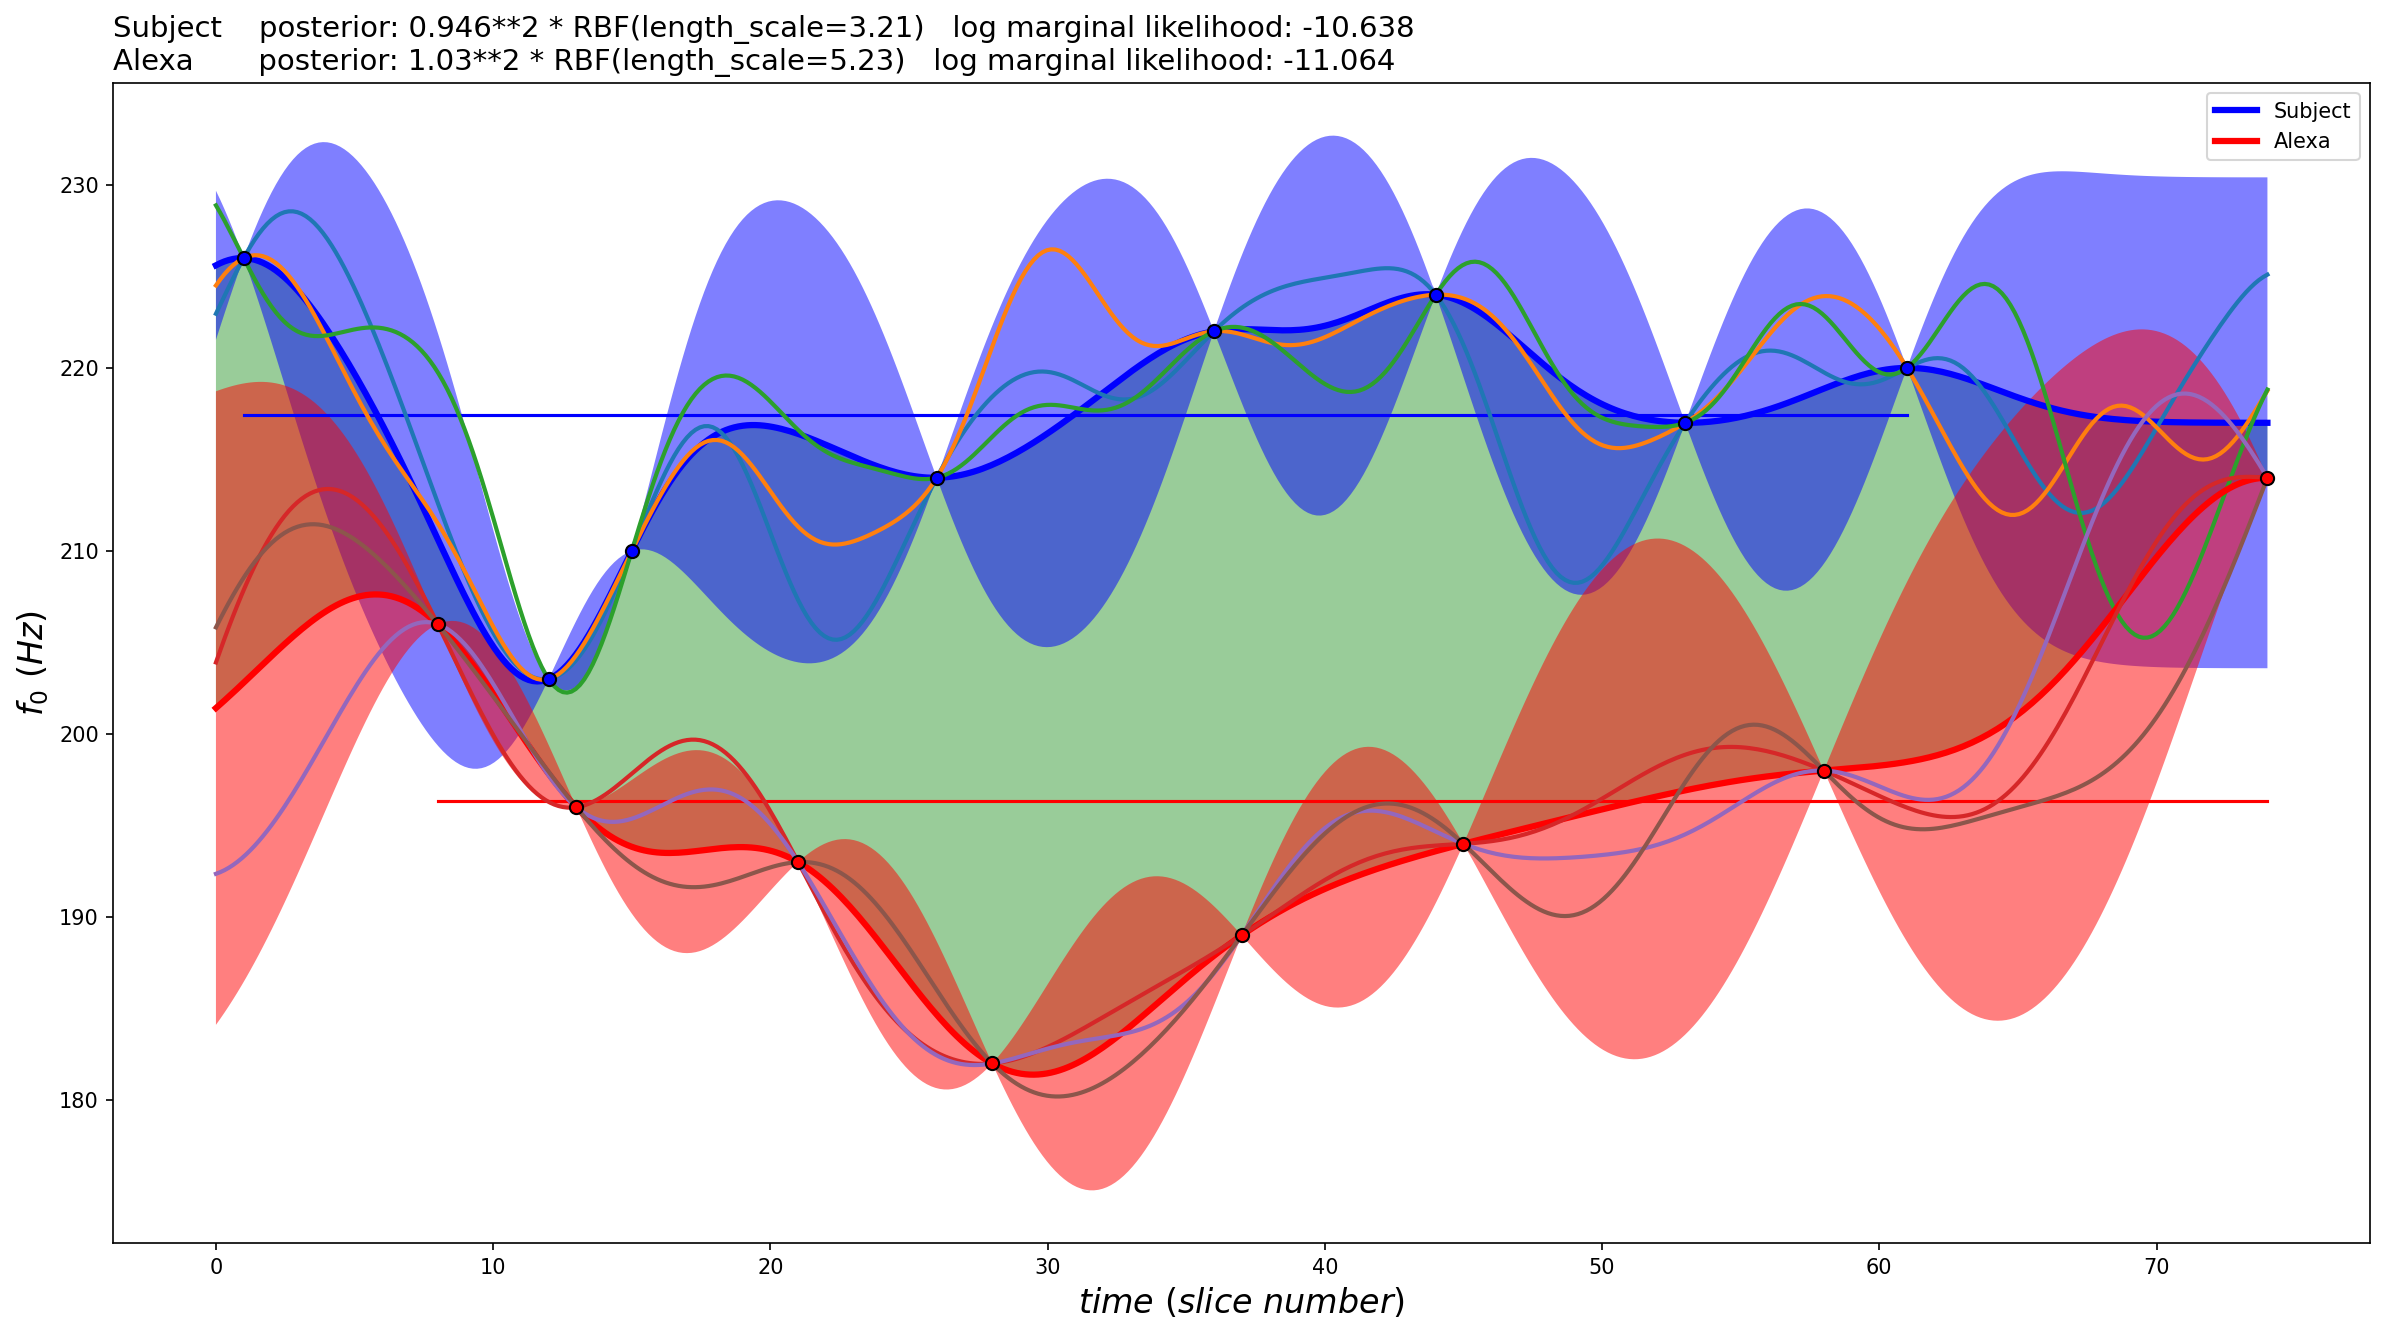
\includegraphics[width=\textwidth]{GP_VACC_with_draws}
	\caption[Gaussian process regression on a conversation with Alexa]
		{Gaussian process regression for an interaction of a participant with Alexa.
		The thick blue and red lines show the predictions' mean.
		The additional lines around the means are randomly drawn functions from the fitted kernel representing potential variational output.
		The colored areas around the means lines show the \SI{95}{\percent} confident interval for the distributions of the same color.
		The straight horizontal lines indicate the overall mean of each speaker's productions.
		The posterior parameters and the log marginal likelihoods of the fitted distributions are stated at the top.}
	\label{fig:gp_vacc}
\end{figure}
%
where $\mu_{\vec{x}}$ is the mean feature value of a single speaker and $\Sigma_*$ is the fitted additive covariance function described in \cref{subsec:covariance_functions}.
It is important to note that the mean is not zeroed (as often done in \ac{gp} regressions), to maintain the original input's mean for the subsequent steps.
The kernel was initialized with the priors $C = 1$, $\ell = 1$, and no assumptions regarding the noise level $\xi$.
The search boundaries for the RBF and noise components were $1 < \ell < 100$ and $\num{1e-4} < \xi < 10$, respectively, with a maximum of six optimization iterations.
% the initial one plus five allowed restarts (n_restarts_optimizer parameter in code)
% \xi is here the sign for noise
The datapoints of the original series were grouped by the turn they belong to.
Then, the average values of turns immediately before and after a floor change were taken as input datapoints for the \ac{gp}.
This results in evidence concentrated around input from the other interlocutor, with the objective to capture turning points that are more prone to accommodation.
With the fitted kernel, a continuous prediction can be made for each speaker over the entire conversation timespan.
\Cref{fig:gp_vacc} shows an example of \ac{gp} predictions for one of the conversations.

\subsection{Marking degrees of change}
\label{subsec:measuring_changes}

Once a regression line is drawn for each speaker from their respective distributions, the differences between the speakers' productions can be measured.
Due to the high temporal resolution used here, more fine-grained degrees of change over time can be calculated.
These differences are calculated by the subtracting the trapped areas between the two regression lines (see \cref{fig:gp_vacc})
%
\begin{equation}
	f_{diff} \equiv\Delta\vec{x}_* =
	\int_{\vec{x}_i}^{\vec{x}_{j}}\mu_{f_*participant} -
	\int_{\vec{x}_i}^{\vec{x}_{j}}\mu_{f_*alexa}
\end{equation}
\eqname{Difference between speakers' \acs{gp} draws}
\noindent
%
and the directional derivatives of the resulted delta line to measure the degree of change
%
\begin{equation}
	\nabla\Delta\vec{x}_*' = \frac{d}{dx}f_{diff}
\end{equation}
%
along the delta line.
\Cref{fig:diff_and_derivatives} illustrates these two measures on the same conversation from \cref{fig:gp_vacc} using the mean prediction of each speaker.
%
\begin{figure}[t]
	\centering
	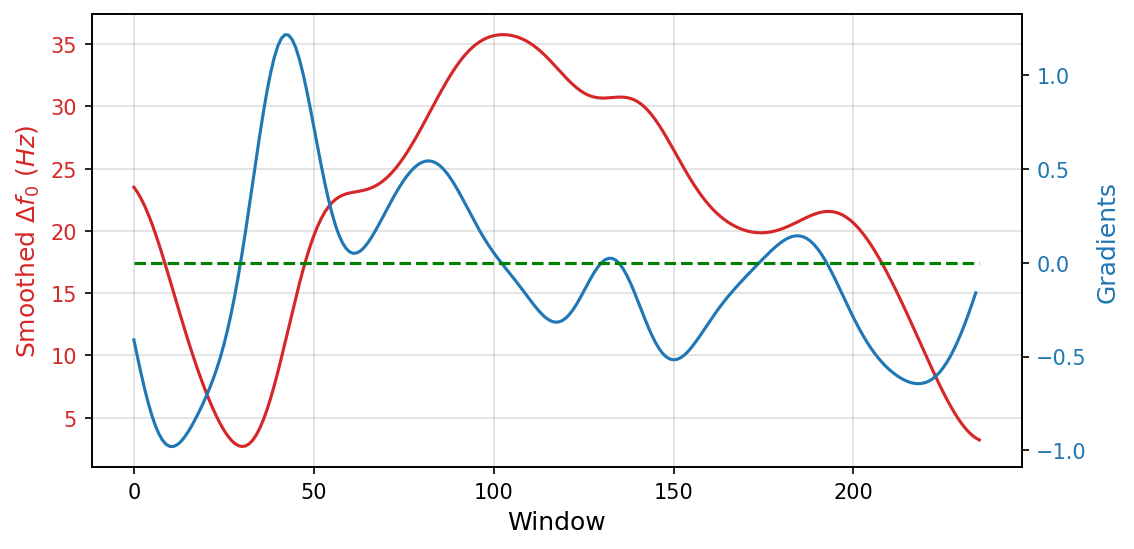
\includegraphics[width=\textwidth]{diff_and_derivatives}
	\caption[Continuous integral differences and derivatives in an interaction]
		{Continuous integral differences (red line) and their corresponding derivatives (blue line) of speakers' productions in a conversation.
		The dashed green line shows the zero-gradient, i.e., no-change threshold.}
	\label{fig:diff_and_derivatives}
\end{figure}
%
For creating a generation process as described in \cref{sec:accommodation_as_a_lm,sec:clustering_and_incremental_generation}, the changes must be marked with pre-defined labels.
To that end, the derivative values were translated into a continuum of change ranging from \textit{divergence} to \textit{convergence}.
Based on this continuum, a discrete scale can be defined.
The more categories this discrete scale offers, the more specific the behavior descriptions can be.
\Cref{fig:cont_disc_scales} shows this process for a discrete scale of three categories: divergence, no (major) change, and convergence.
%
\begin{figure}[t]
	\centering
	\subfigure[Continuous scale]
		{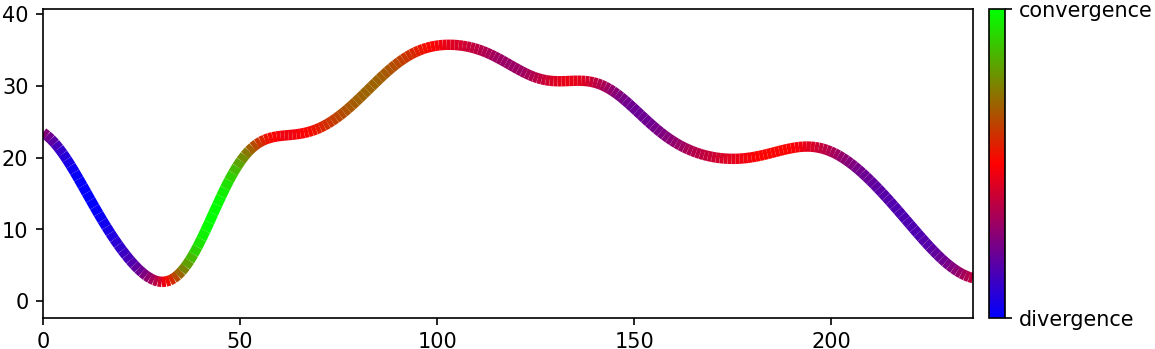
\includegraphics[width=0.47\textwidth]{cont_scale}
	\label{fig:continuous_scale}}
	\hfill
%	\vspace{-1cm}\hfill\hspace{-1cm}{\hbox{\LARGE $\Longrightarrow$}}\hfill
	\subfigure[Discrete scale]
		{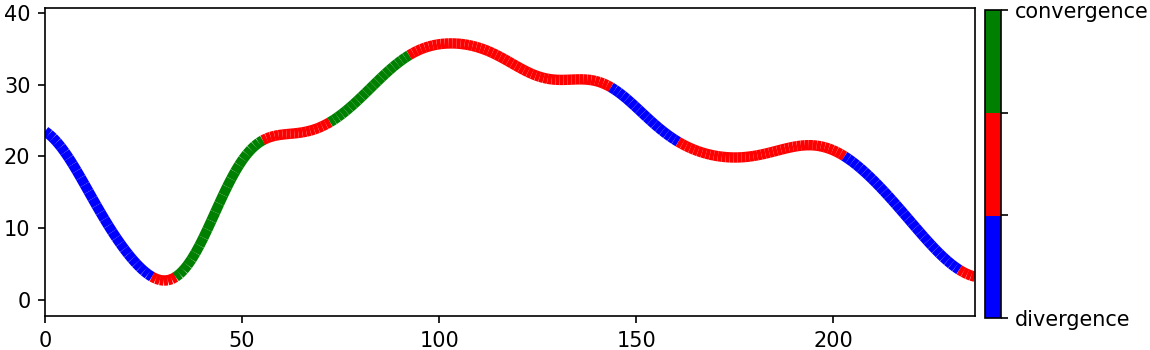
\includegraphics[width=0.47\textwidth]{discrete_scale}
	\label{fig:discrete_scale}}
	\caption[Continuous and discrete scales for labeling degrees of change]
		{Continuous and discrete color-coded scales for labeling degrees of change in a conversation.}
	\label{fig:cont_disc_scales}
\end{figure}
\todo[inline]{need more details regarding how the discrete categories are defined?}

\section{N-gram representation for accommodation sequences}
\label{sec:accommodation_as_a_lm}

In order to generate accommodation sequences, a model that can iteratively emit labels based on the label history is needed \citep[in contrast to, e.g., models with the Markov property, as in][]{Bellman1957markovian}.
%Predictions of any model based on Markov decision process depend only on the current state of the conversation.
%This neglects the temporal aspect of the conversation.
%One way to overcome this is to extend the transition function of a Markov-based model, so that the previous $n$ states are somehow incorporated into the action $a$ of $P_a(s, s')$.
%However, this violates the core idea of a Markov decision process and makes it more complicated to use.
An n-gram model is proposed here, which incorporates a portion of a sequence's history (\emph{context}).
The estimation of the element $e$ at position $i$ is calculated by the probability term $P(e_i \mid e_{i-n},\ \ldots\ , e_{i-1})$.
N-gram models are traditionally used for describing sequences of linguistic units, like words in a language model \citep[e.g.,][]{Niesler1996variable}, and are used in applications with sequential nature, like machine translation \citep{Marino2006ngram} and proteins identification \citep{Xu2015identification}.
The n-grams model here describes sequences of \emph{accommodation levels} in a conversation.
These levels are represented by discretized values that are based on the degrees of change acquired in \cref{subsec:measuring_changes}.
After computing the n-grams probabilities of the level, this model can be used for generating new sequences.
The resolution and variability of the model can be controlled by changing the n-grams' $n$ and the number of levels used to distinguish between the different accommodation levels.

\subsection{Dimensionality reduction and symbolic representation}
\label{subsec:dim_reduction_and_symbolic_rep}

\begin{figure}[t]
	% 20171130A_Quiz_01 was used for these figures
	\centering
	\subfigure[\acs{paa} of the original time seires.
			   The blue continuous line shows the z-normalied original time series of mutual change gradients in a conversation, which was extracted as described in \cref{subsec:measuring_changes}.
			   The organe circles show the \acs{paa} points created based on the continuous lines.
			   The dashed orange line is the linear interpolation between the \acs{paa} points.
			   Note that this lines is for illustration only and is not taken into account in the analysis.]
		{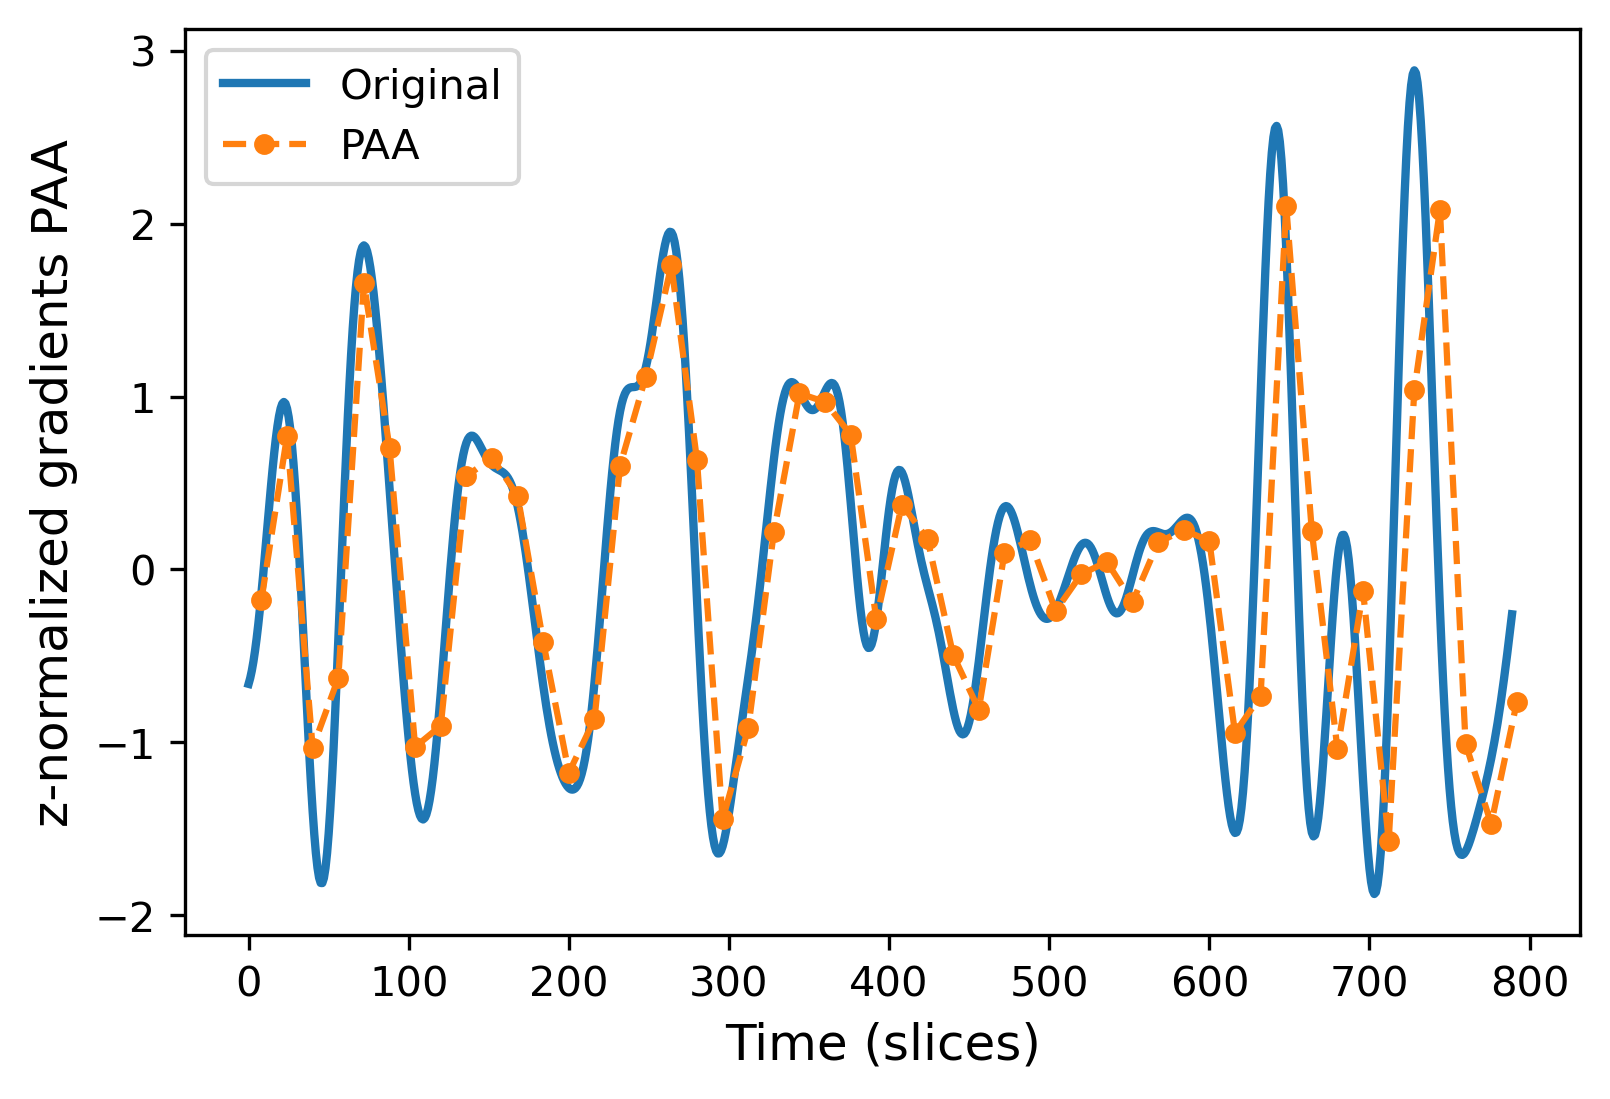
\includegraphics[width=0.47\textwidth]{PAA}
	\label{fig:paa}}
	\hfill
	\subfigure[\acs{sax} of the \ac{paa} values.
			   The blue circles are the \acs{paa} points from \cref{fig:paa}.
			   The blue line visualizes the linearly interpolated trend of these points.
			   The horizontal green dashed lines show the margins of the five bins that split the points discrete bins derived from a normal distribution.
			   The organe labels (\enquote*{d+}, \enquote*{d}, \enquote*{n}, \enquote*{c}, and \enquote*{c+}) mark the classification of each point based on the bin it falls into.]
		{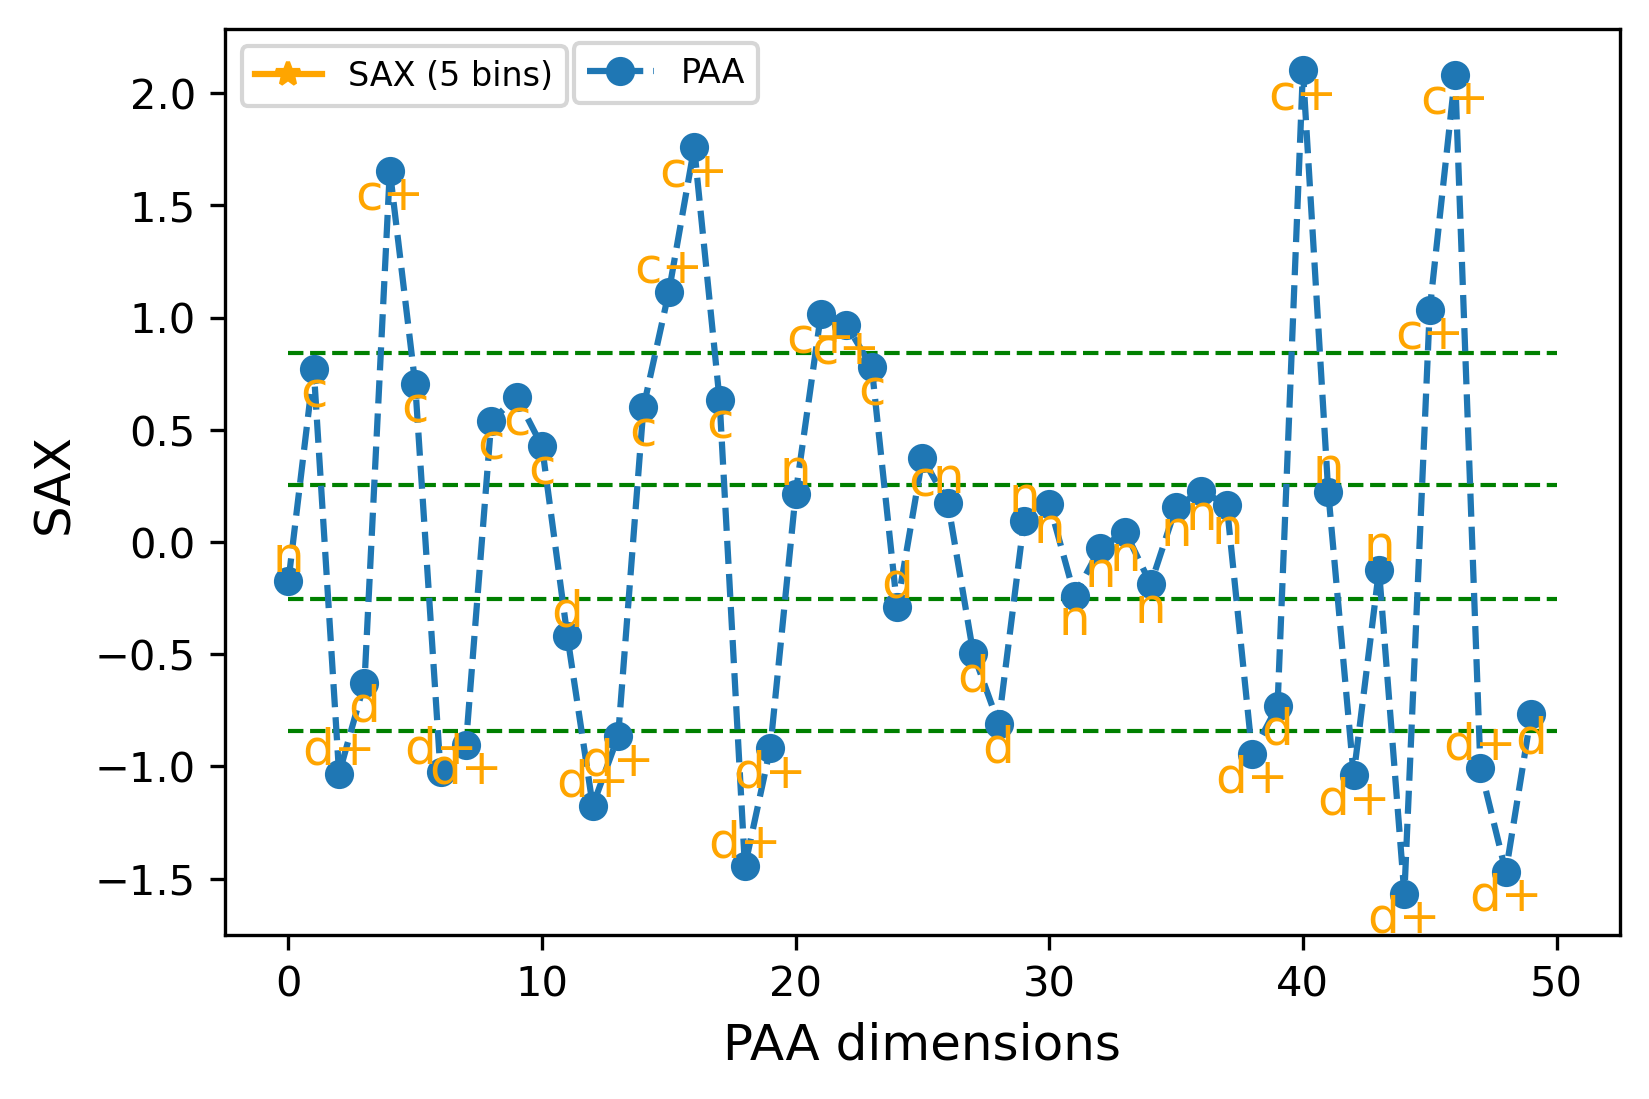
\includegraphics[width=0.47\textwidth]{SAX}
	\label{fig:sax}}
	\caption[\acs{paa} and \acs{sax} of the time series representation of a conversation]
		{\Ac{paa} and \ac{sax} of the time series representation of mutual change in a conversation.}
	\label{fig:paa_and_sax}
\end{figure}

The time series gradient extraction process described in \cref{subsec:measuring_changes} is greatly high dimensional, even for short interactions.
While this representation is useful for gaining a fine-grained overview of the data, it is not practical for various analysis techniques that do not benefit from (or are not designed to handle) such high-dimensional data.
For instance, clustering algorithms, which need to iteratively compare between all points in a collection, scale better with lower dimensionality.
The dimensionality of the data in question here is reduced using \acl{paa} \citep[\acl{paa};][]{Keogh2001dimensionality}, which is a common dimensionality reduction technique for time series.
\Cref{fig:paa} shows the output of \ac{paa} on the gradients of an interactions.
Each element $\vec{x}_i$ of the reduced vector is calculated by
%
\begin{equation}
	\label{eq:paa}
	\vec{x}_i = \frac{N}{n} \sum_{j=\frac{n}{N}(i-1)+1}^{i(\frac{n}{N})} S_j,
\end{equation}
\eqname{\Acl{paa} dimensionality reduction}\noindent
%
where $n$ is the dimensionality of the original times series, $1 \leq N \leq n$ is the dimensionality of the output vector, and $S_j$ is the $j$\textsuperscript{th} element of the original time series.
\Ac{paa} is suitable here, as the goal is to obtain vectors with fewer dimensions that still faithfully represent the data, and not, e.g., decompositions of the original data \citep[cf.\ method survey in][pp.~271-275]{Keogh2001dimensionality}.
Since the goal here is to compare \emph{trends in change} within and across conversations rather than their absolute values, all gradient time series where z-normalized before applying the \ac{paa}.
In the context of conversation analysis, the \ac{paa}'s dimensional cardinality determines the \enquote{zoom} level, i.e., how fine-grained the representation is (the more points the more in detail the time series is described).
Ultimately, \ac{paa} provides \textbf{continuous numeric values} that represent the overall shape of the original time series.

\Ac{paa} is suitable for analyses of continuous numeric values.
However, discrete values are required for symbolic n-gram sequences.
For converting the continuous \ac{paa} values, the \acl{sax} \citep[\acs{sax};][]{Lin2007experiencing} method was used.
\Ac{sax} assigns a string label based on a pre-defined number of bins, as shown in \cref{fig:sax}.
Such labels provide a more meaningful and compact representation.
As explained by \citet{Apostolico2003monotony}, it is preferable to use a discretization technique that uses a symbol set with equiprobability.
%\footnote{It can be claimed that realistically equiprobability does not hold for the symbols in this kind of data.
%While that may be true to some extent, neither the pre-processing nor the dimensionality reduction steps held any assumptions regarding the values in each \ac{paa} sequence.
%Moreover, the data was z-normalized to avoid any bias stemming from specific numeric values.
%For these reason, together with the fact that the participants were, in practice, free to speak in whatever way they wanted, equiprobability can be assumed in this analysis.
%See \cref{subsec:word_extraction_and_seq_prob} for more information regarding the distribution of extracted symbol sequences}.
To that end, the \ac{sax} discretization was done using bins based on the normal distribution of the z-normalized values.
% this is defined by the method="normal" parameter in the SAX function (or `strategy` parameter internally)
Five bins, representing accommodation levels, are used here for categorizing degrees of change, labeled \enquote*{d+} for \emph{strong divergence}, \enquote*{d} for \emph{divergence}, \enquote*{n} for \emph{no (major) change}, \enquote*{c} for \emph{convergence}, and \enquote*{c+} for \emph{strong convergence}.
This number of bins was found to adequately describe types of accommodation;
three labels resulted in underspecified sequences where all degrees of convergence or divergence are labeled similarly, and seven or more labels did not provide substantial additional insights and often yielded sparse sequences.
The motivation for choosing an odd number of labels is to have a neutral (\enquote{no-change}) label and even number of labels for convergence and divergence, due to the assumption that they are equally likely to occur.
However, an even number can be used as well, forcing each value to stand for either convergence or divergence while ignoring zero values.
It is also possible to allocate more labels to convergence or divergence, if one of them is assumed to occur more in the data and a more fine-grained description of it is desired.
Note that the term \emph{synchrony} is avoided here for describing a steady distance between the speakers, as per its definition in \cref{subsec:variation_types} it entails additional properties regarding the individual change of each speaker.
Ultimately, \ac{sax} provides \textbf{discrete textual labels}, which provide a discretized version of the original time series.

\subsection{Sequence extraction and probability calculation}
\label{subsec:word_extraction_and_seq_prob}

%\begin{figure}
%	\centering
%	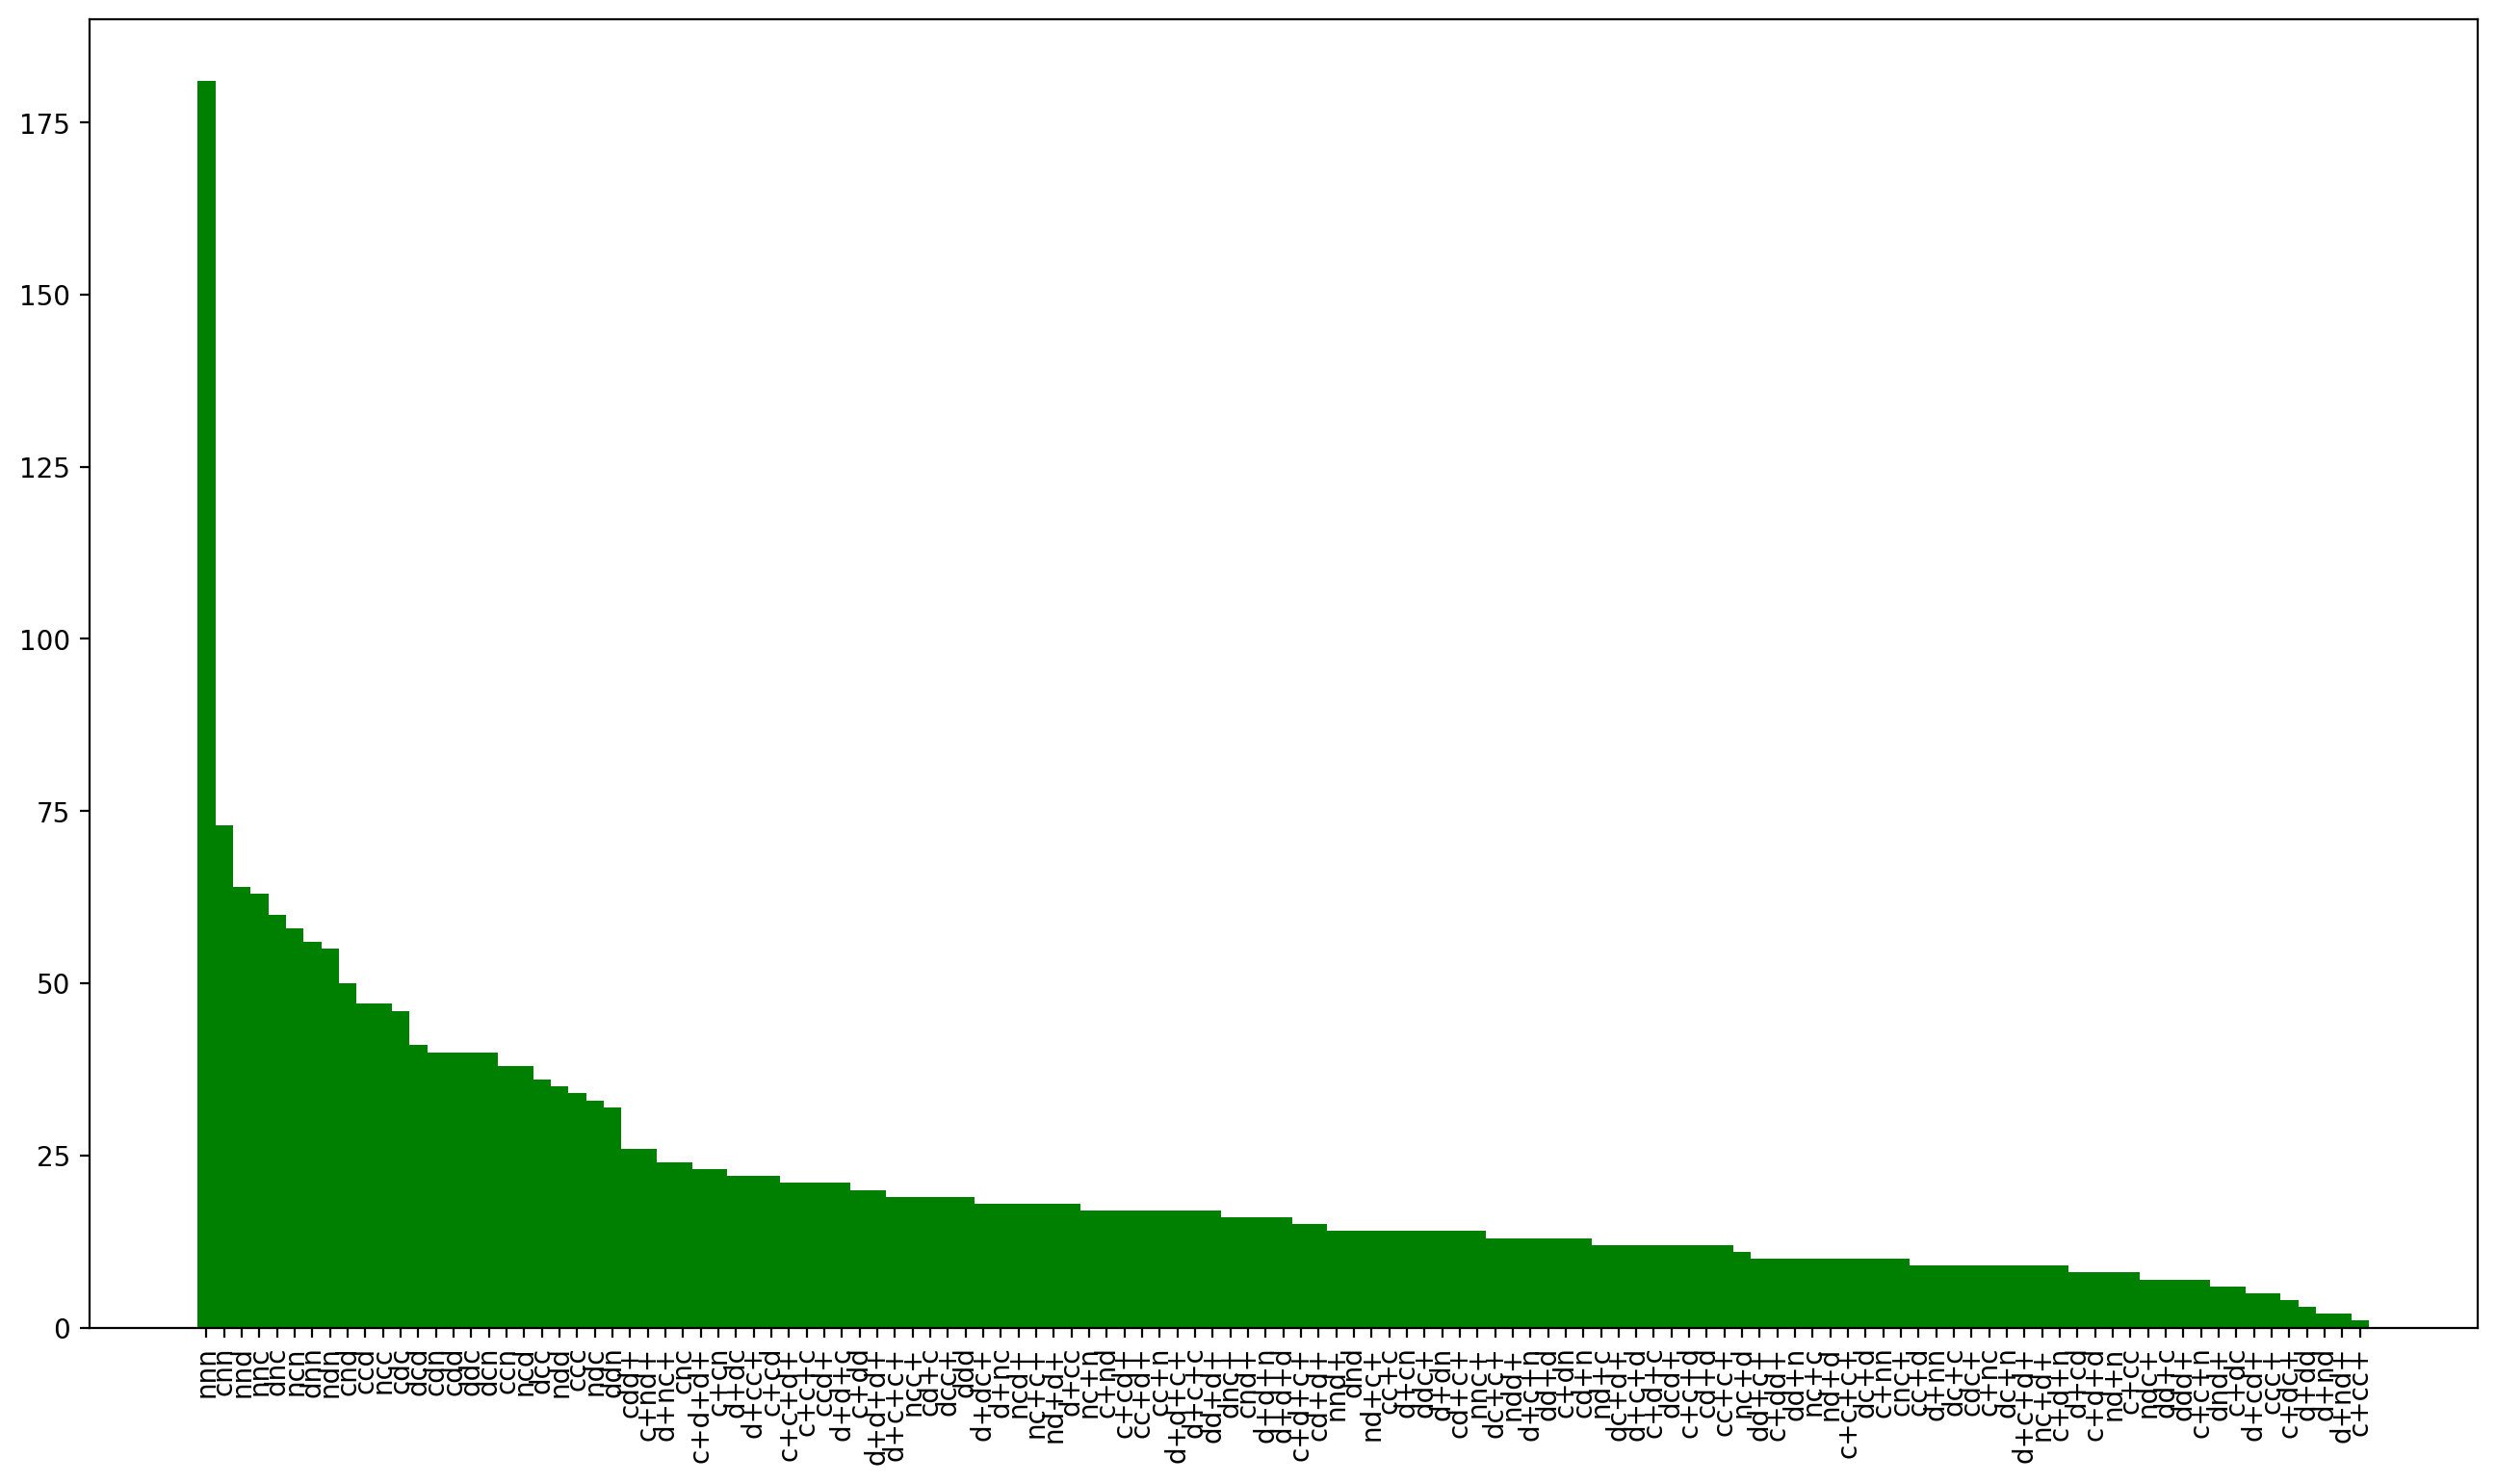
\includegraphics[width=\textwidth]{accomm_symbols_dist}
%	\caption[]
%		{}
%	\label{fig:accomm_symbols_dist}
%\end{figure}

After applying \ac{sax}, a sequence of accommodation labels is obtained for each corresponding interaction.
The count distribution of the labels was computed to examine their frequency.
As expected, the symbol $n$ had the highest frequency, about 2.5 times higher than the convergence and divergence labels $c$ and $d$, whose frequency, in turn, was roughly four times higher than the frequency of the strong convergence and strong divergence labels $c+$ and $d+$.
The same calculations were repeated for sub-sequences of the labels as they appear in the \ac{sax} sequences.
The frequencies can be divided into three groups: matching the trend of the single-label distribution, repeated $n$ labels were about three times more frequent than the second group, which consisted of most other sub-sequences that included $n$.
Lastly, this group was followed by a long tail of less frequent sequences, starting from counts three to four times lower, which included the rest of the symbol combinations within a sub-sequence.
Sub-sequences with many repeated $c+$ or $d+$ labels (i.e., sustained convergence/divergence) mostly appeared toward the end of the tail.
Increasingly smoother instances of the same overall distribution shape were found for all sub-sequence lengths from two and up to half the \ac{sax} sequence length (after which such frequencies become not as meaningful).

\begin{table}[t]
	\centering
	\caption[Examples of probabilistically generated accommodation level sequences]
		{Three examples of probabilistically generated accommodation level sequences.
		 Each sequence consists of eight labels that were generated based on the initial context of the padding symbol $p$.
		 The first line of each example shows the generated symbols as explained in \cref{subsec:dim_reduction_and_symbolic_rep} and their average variability (value between 0 and 1, higher number means more variability.).
		 The second line lists the probability of each generated label given the context seen up to that point and the overall probability of generating this entire sequence.
		 In the third line are the perplexity scores of the trigrams ending with the corresponding generated label given the context at the time of the generation.
		 Note that the first two padding labels do not have any scores, since they are given as the initial context.
		 Similarly, the first generated label does not have a perplexity score, as it can only be calculated once the sequence is longer than the one trigram.}
		 % variability was calculated as the average "deviation", where c and d have value of 0.5, c+ and d+ value of 1, and n value of 0, for Example (c + c+ + n + n + d+ + c + n + n) / 8 = 0.375
	\label{tab:generated_symbol_sequences}
	\begin{tabularx}{\linewidth}{*{10}{c}l@{\hskip 0.1cm}l}
		\toprule
		p    & p    & n    & n    & n    & c    & n    & d    & d    & c    & variability: & \num{0.187}  \\
		---  & ---  & 0.44 & 0.46 & 0.55 & 0.18 & 0.32 & 0.29 & 0.25 & 0.35 & probability: & \num{1.63e-4}\\
		---  & ---  & ---  & 2.22 & 1.99 & 3.16 & 4.16 & 3.27 & 3.67 & 3.35 & perplexity: & \num{3.11}   \\[0.4cm]
		
		p    & p    & n    & d    & d    & c    & c+   & d+   & d+   & c+   & variability: & \num{0.687}  \\
		---  & ---  & 0.44 & 0.17 & 0.25 & 0.35 & 0.13 & 0.25 & 0.34 & 0.19 & probability: & \num{1.37e-5}\\
		---  & ---  & ---  & 3.67 & 4.88 & 3.35 & 4.69 & 5.62 & 3.46 & 3.96 & perplexity: & \num{4.23}   \\[0.4cm]
		
		p    & p    & c    & c+   & n    & n    & d+    & c     & n    & n    & variability: & \num{0.375}  \\
		---  & ---  & 0.30 & 0.25 & 0.25 & 0.16 & 00.04 & 00.20 & 0.22 & 0.41 & probability: & \num{2.16e-6}\\
		---  & ---  & ---  & 3.67 & 4.03 & 5.02 & 12.72 & 11.51 & 4.77 & 3.30 & perplexity: & \num{6.43}   \\
		\bottomrule
	\end{tabularx}
\end{table}

To calculate label probabilities, these sub-sequences were treated as n-grams with $n = 3$, i.e., trigrams.
Similar to an n-gram language model, the size of the n-gram determines the amount of previously acquired evidence taken as context when calculating the probability of the a subsequent label.
This fulfills a similar role as the \emph{pool size} parameter of the computational model (see \cref{sec:parameters}).
In both cases, the goal is to consider the temporal evolution of the conversation for predicting its continuation.
To account for conversation-initial sequences, the beginning of each symbol sequence was padded.
The end of the sequence is not padded, since, unlike a traditional language model, the generation process here assumes that the user decides when to end the interaction and therefore does not attempt to predict it.
This summed up to a collection of \num{2700} trigrams from all interactions, which comprised 143 (\SI{92}{\percent}) out of the $5^3$ +~1~$\times$~5~two-padding +~5~$\times$~5~one-padding $= 155$~possible label combinations.
% 2700 is 54 solo interactions times 50 trigrams for each: the size of SAX used was 50, which gives 48 trigrams. with the 3 trigrams added from padding, it's 50. 50 times 54 = 2700
This shows a great variety of conversation dynamics.
% however, since not all possible combinations are used for training, unseen trigrams can still be seen during generation. we set the vocab to be all possible combinations (plus all initial padded trigrams)
% smoothing??
% probabilities for OOV trigrams?
Based on these n-grams, sequences of symbols, representing accommodation levels in a conversation, can be probabilistically generated.
The predicted accommodation label $l$ after two observed convergence labels $c$ is taken from the probability distribution $p(l \mid c,\ c)$.
\Cref{tab:generated_symbol_sequences} shows examples of such probabilistically generated sequences for the first eight accommodation labels of a conversation.
The variability measure is defined as
%
\begin{equation}
	P(sequence) = \frac{1}{N} \sum_{i=1}^{N} \left| \frac{num(label_i)}{2} \right|,
	% the absolute value is divided by 2 to make the vaerage per turn (i.e., max 1 "variability point" per turn)
\end{equation}
\eqname{Label sequence variability score}
\noindent
%
where $N$ is the number of labels in the sequence and $num(label)$ maps a label to a numeric value between -2 ($d+$) and 2 ($c+$).
The overall probability of the sequence is calculated by
%
\begin{equation}
	sequence\ probability = \prod_{i=3}^{N} p(label_i \mid label_{i-2}, label_{i-1}).
\end{equation}
\eqname{Label sequence probability score}
\noindent
%
The perplexity measure is the average of all perplexity scores of the individual labels in the sequence.
It is worth noticing that the third sequence in the table has lower variability than the second, although its overall probability is lower and its mean perplexity is higher.
That means that, based on this model, higher variability is sometimes the more likely evolution of in interaction.
On the other hand, since in most contexts, the probability of label $n$ is relatively high, sequences with more no-change predictions are more likely to be generated, on average.

\section{Clustering and incremental variational generation}
\label{sec:clustering_and_incremental_generation}

To achieve the goal of the generating behaviors based on extracted core behaviors, the behavior description method from \cref{subsec:measuring_changes} and the n-gram approach from \cref{sec:accommodation_as_a_lm} need to be combined.
On top of this, turn-level variations can be introduced using the \acp{gp}, as explained in \cref{sec:time_series_analysis}.
This will result in a variational probabilistic generation based on core behaviors detected in the dataset.

First, clusters of participant behaviors are sought to detect general similarities in behavioral patterns.
Two clustering methods were utilized, namely k-means and hierarchical linkage, each offering different insights on the data.
The former method is a top-down approach with a pre-defined number of clusters, which offer a more general view on the patterns, and the latter is a bottom-up approach with no prior assumptions, where more individual differences can be observed.
While it cannot be expected to find a completely distinct pattern for each speaker, some separable clusters and general tendencies are expected to emerge, both when inspecting individual speakers and the dataset as a whole.
%
\begin{figure}[t]
	\centering
	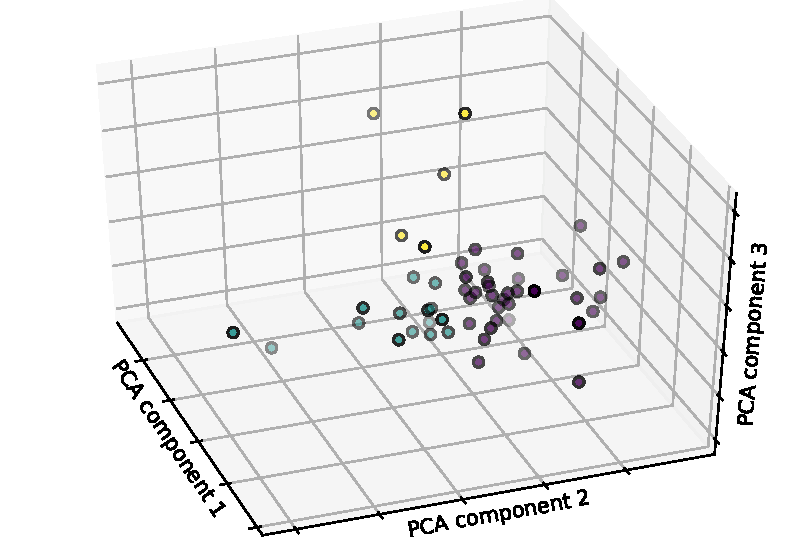
\includegraphics[width=\textwidth]{3d_clustering}
	\caption[3D \acs{pca} components projection of accommodation changes clustering]
		{k-means clustering of the first three \acs{pca} components of the interactions' \acs{paa} sequences.
		Each circle represents one sequence in the three-dimensional space.
		A circle's color indicates the cluster to which the datapoint belongs.}
		% elevation is 40 azimuth is 160
	\label{fig:k-means_clustering}
\end{figure}
%
To determine the number of clusters $k$ and the number of projection dimension $d$, the the clustering process was performed with two, three, and five clusters using the two and three first \ac{pca} components.
The process was repeated 10 times to account for the algorithm's non-deterministic nature, with the combination of three clusters and three components best separating the data, on average.
The resulted clusters are shown in \cref{fig:k-means_clustering}.

\afterpage{%
	\begin{landscape}
		\begin{figure}[t]
			\centering
			\hspace*{-4.7cm}
			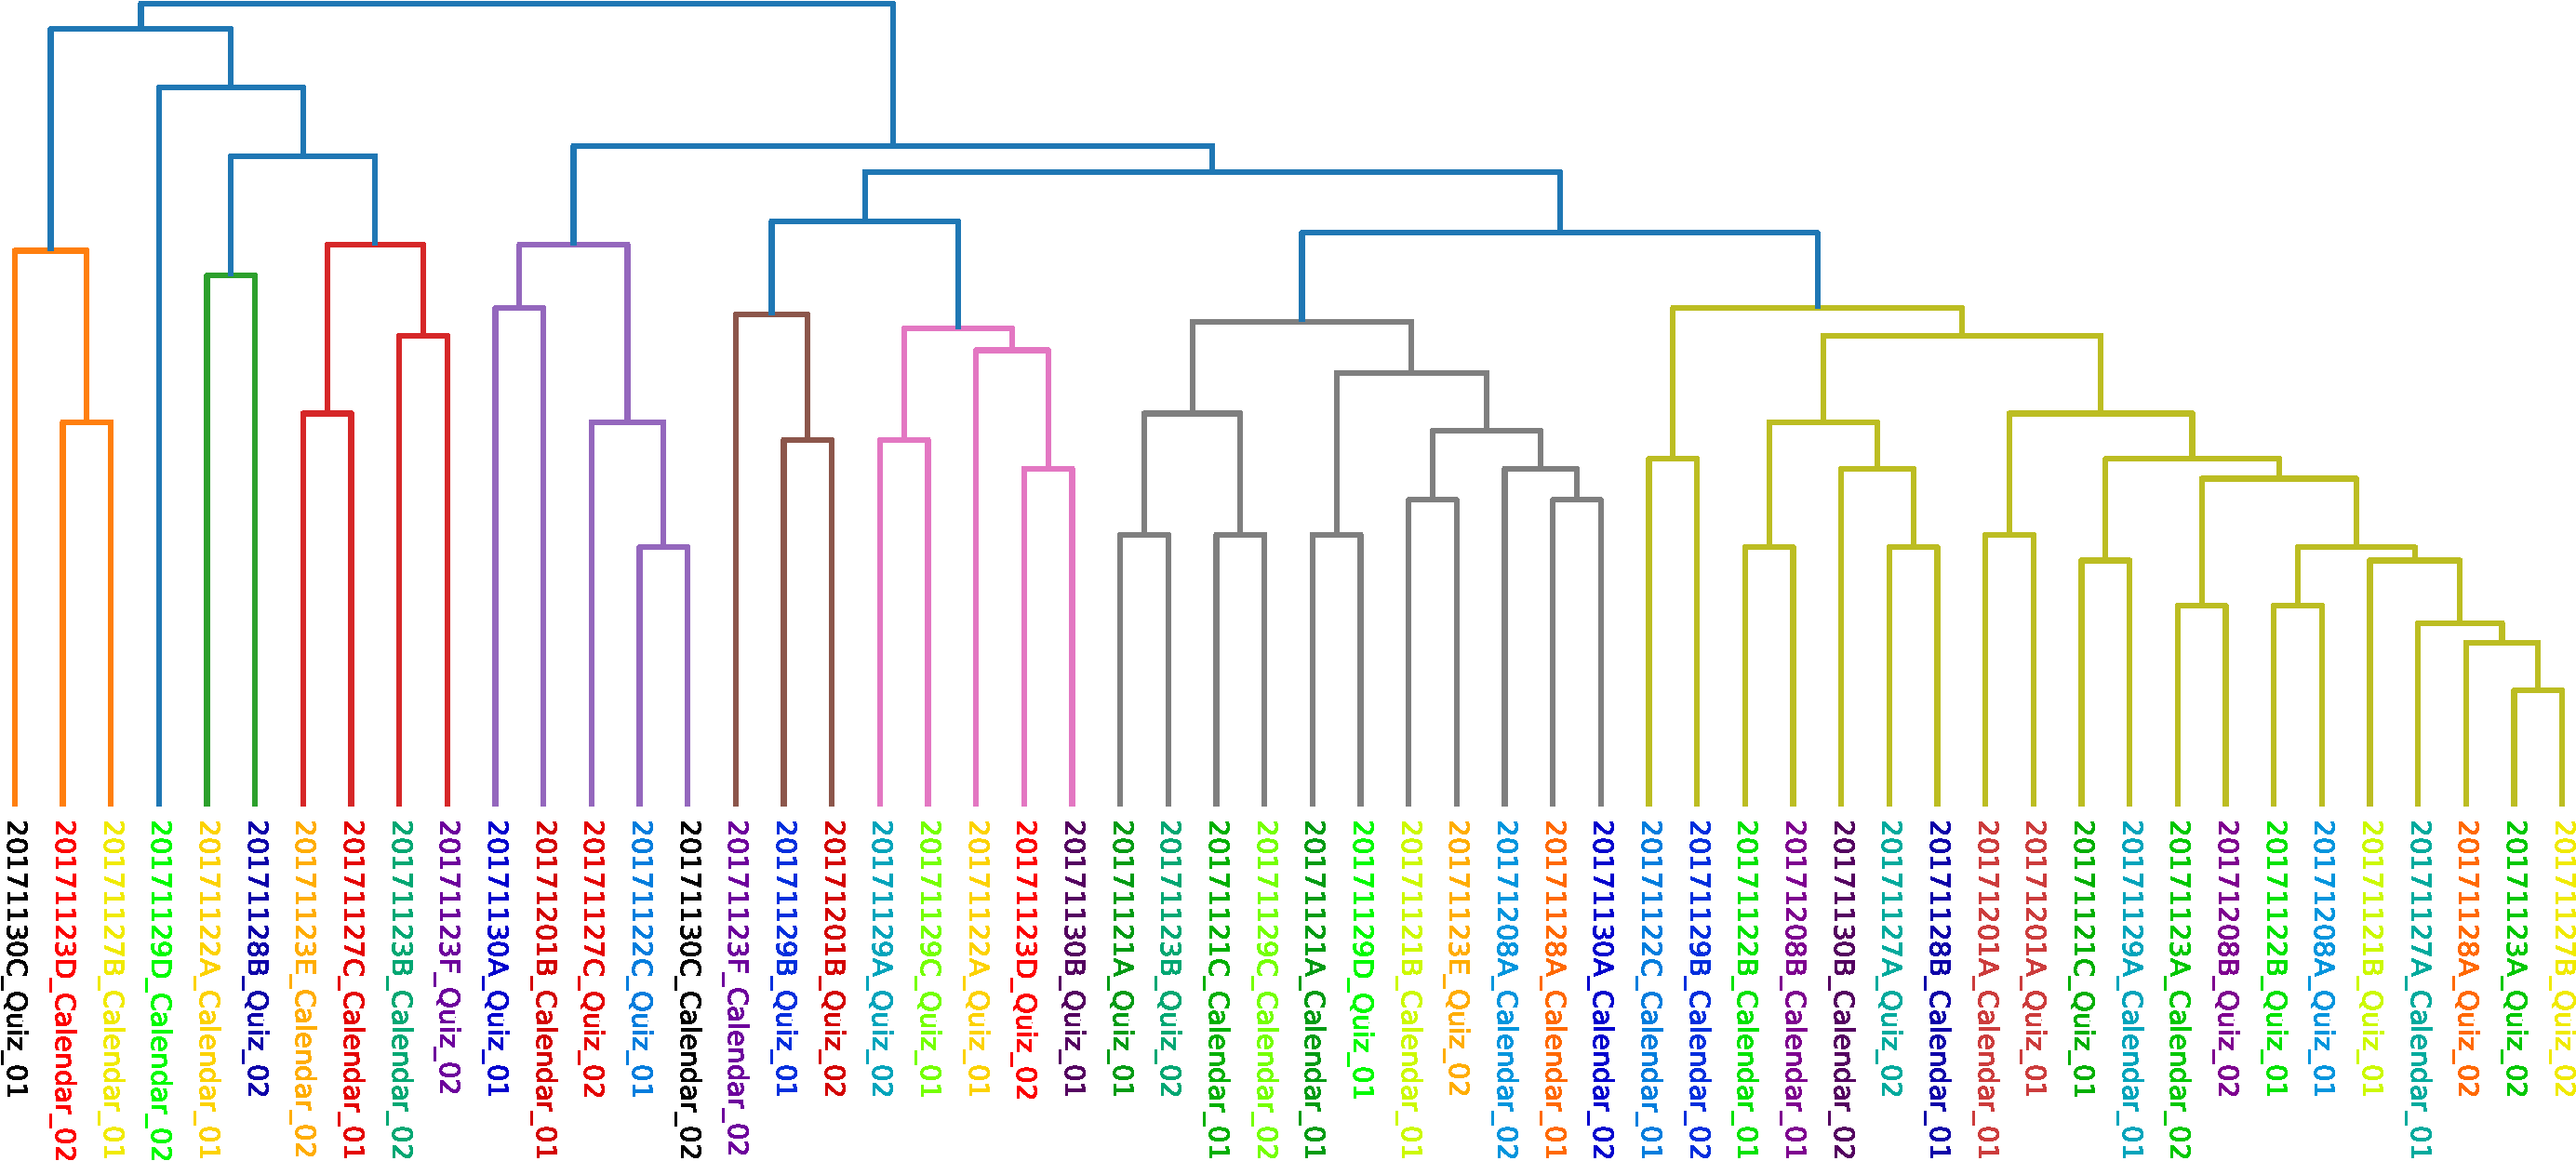
\includegraphics[width=1.65\textwidth]{paa_dist_dendrogram}
			\caption[Dendrogram of time series \acs{paa} representation of interactions distances]
				{Dendrogram of the time series \acs{paa} representations of the interactions based on complete-linkage distances.
				Each cluster is represented by a different color of lines.
				% Blue lines connect pairs of clusters that are most similar to each other, and similarly pairs of the closest subsequent sub-cluster and eventually leaves are connect directly to each other.
				Each leaf represent the interaction indicated by its label.
				Each participant's interactions pair is marked by labels of the same color.
				The leaf and cluster colors are \emph{not} related.
				The leaves are order horizontally by their distance from left to right, so that the leaves of interactions that are more similar to each other (both inter- and within-cluster) are positioned closer.
				For example, the two interactions of participant \texttt{20171201A} (12\textsuperscript{th} and 13\textsuperscript{th} leaves from the right) are the closet to each, as they are positioned together and within the same smaller sub-cluster.
				Contrarily, the labels of participant \texttt{20171128B} are positioned the furthest from each other (6\textsuperscript{th} and 41\textsuperscript{st} leaves from the left).}
			\label{fig:paa_dist_dendrogram}
		\end{figure}
	\end{landscape}
}

While top-down clustering uncovers general grouping of the interactions in the dataset, bottom-up hierarchical clustering can reveal structural relations between them and measures their degrees of similarity.
The distances between the 54 interactions can be measured and compared using their \ac{paa} values, as calculated in \cref{subsec:dim_reduction_and_symbolic_rep}.
The calculation was done using the \emph{complete linkage} agglomeration technique (a.k.a.\ farthest point algorithm).
This use of this linkage is motivated by the assumption that there are more general behavioral patterns to find beyond the speakers' individual behaviors, as it searches for the most dissimilar (and hence principally all) interactions in neighboring clusters and not only the closest one (single linkage).
This method also allows using the entire \ac{paa} vectors without any pre-processing.
\Cref{fig:paa_dist_dendrogram} shows the bottom-up distance clustering based on this linkage.
Although, unsurprisingly, no definite order emerges, some general trends can be seen regarding the similarity between interactions of the same human speaker.
Seeing that leaves are ordered horizontally based on their overall similarity, the distances between their positions can be utilized to determine each participant's behavior consistency.
The average distance of the population is 16.5, far from the maximal possible average of 27, which points to a general tendency of speakers to behave similarly in their conversations.
% This is the maximal possible average, since this is when each interaction is half of the population away from its pair.
% With the largest possible distance between two leaves being 53, the space can be divided into three bins of 18 (rounded up).
To reinforce this claim, dividing the space into three equal bins of \enquote{short}, \enquote{medium}, and \enquote{long} distances shows that 16, 10, and 1 interaction(s) fall into these bins, respectively.
Moreover, this distribution has a median of 16 and its second tertiles located at 19, far from the \enquote{long distance} bin.
Such skewness in the distribution indicates that speakers' behaviors are more often than not similar across interactions, regardless of any other factor (interaction length, task, order, and other factors discussed in \cref{chap:speech_variations_in_hhci}).
Notably, the two interactions of one participant, \texttt{20171201A}, even have the minimal possible distance of 1 between them (12\textsuperscript{th} and 13\textsuperscript{th} leaves from the right in \cref{fig:paa_dist_dendrogram}) and they are in the same lowest-level sub-cluster.

These clustering techniques show that different accommodative behaviors among speakers can be found and compared.
Together with the probabilistic approach presented in \cref{subsec:word_extraction_and_seq_prob}, these can be used for generating sequences based on a specific behavior -- or rather a group of latent behaviors.
Ultimately, this would result in the system having a \emph{core behavior} with \emph{variations}, per the description in \cref{subsec:variation_types}.
To this end, an \emph{incremental} generation process is needed.
As opposed to the generation process demonstrated in \cref{tab:generated_symbol_sequences}, where the data for the entire interaction was known, an incremental generation is introduced here.
An incremental generation better represents a live interaction, in which only the evidence accumulated up to a certain turn can be used for analysis and prediction of the next turn.
This can be utilized both for integration into a system and for simulating possible system behaviors for research.
%
\begin{figure}[t]
	\centering
	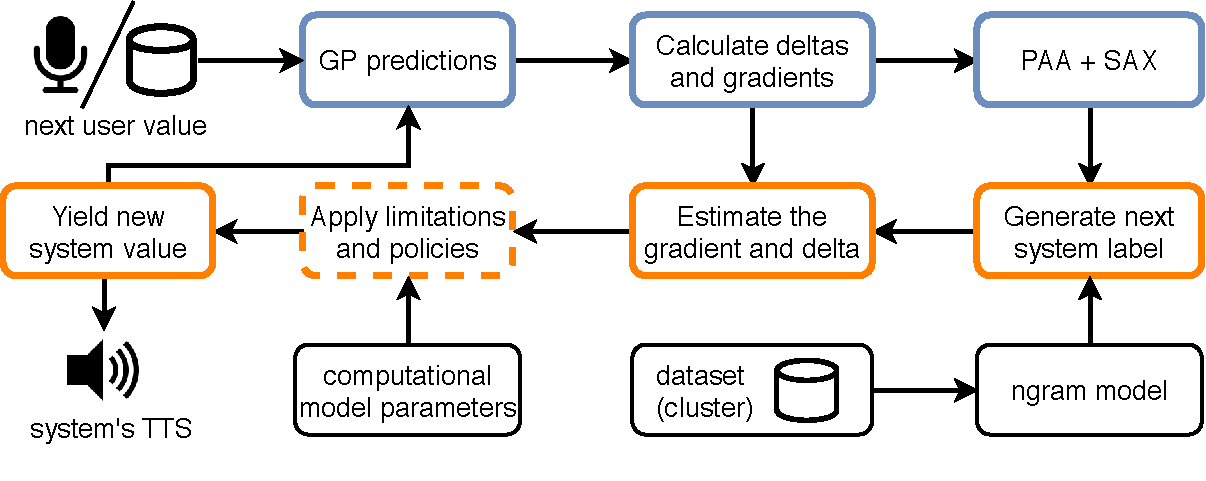
\includegraphics[width=\textwidth]{incr_gen_pipe}
	\caption[Incremental generation process]
		{Schema of the incremental generation process.
		 Blue boxes are related to the user phase and orange boxes to the system phase.
		 Together, they complete a cycle of one round.
		 The dashed orange frame marks an optional step.
		 Note that the new value generated for the system is used both as output (e.g., for \ac{tts} synthesis) and as additional evidence for the next cycle.
		 The user's values can be obtained either from online input or from some database.}
	\label{fig:incr_gen_pipe}
\end{figure}
%
The process is summarized in \cref{fig:incr_gen_pipe}.
It consists of the user and the system phases, which are roughly symmetric and with opposite goals:
While the former assigns a label to an input value, the latter yields a value based on a label (which, in turn, is generated based on the label assigned to the user's input).
A round is completed each time both phases were executed once.
Hence, each round adds two values and their two corresponding labels, one for the user and one for the system.
In the user phase, the latest system output and the new user input -- obtained either from live input or a database -- are added to the rest of the so-far accumulated evidence of their respective \acp{gp}, as done in \cref{subsec:interploating_data_using_kriging}.
Then, deltas and gradients of these values are calculated (\cref{fig:diff_and_derivatives}) to subsequently create \ac{paa} and \ac{sax} sequences (\cref{fig:paa_and_sax}).
The system phase starts with the \ac{sax} sequence contains one label per turn, including the user's new turn.
The next system label is generated using the n-gram model with the probabilities acquired from the subset with the desired accommodative behavior (here, a cluster from \cref{fig:k-means_clustering}).
This label represents a relative z-normalized change degree.
Therefore, the value range covered by this label can be computed from all accumulated gradients, as indicated by the arrow between the second user step to the second system step in \cref{fig:incr_gen_pipe}.
The system's \ac{gp} from the first step is used to draw a single gradient value from that range.
These two steps grant the variational property to the generation process; a label for the overall accommodation direction and a value for the specific amount of change.
The drawn gradient value and the last system's gradient are used to determine the new gradient, from which the next system value can be calculated.
% this step is simply taking the drawn - current to get the difference, which is the amount of change the system shows. the specific value is calculated by this multiplied by the z-normalized value of the lable's bin.
The yielded value is then added to the accumulated evidence, so that it can be taken into account in the user phase's first step of the next round.
In parallel, it can also be used as additional input for a \ac{tts} module of a \acl{sds}, as demonstrated in \cref{sec:architecture_sds,fig:adaptation_module_architecture}.
External limitations or policies can intervene in this step to shape the system's output (see \cref{subsec:assign} for more motivation and examples).
This combination of the statistical and computational models is further explored in \cref{subsec:comb_comp_stat_models}.

\begin{figure}[t]
	\centering
	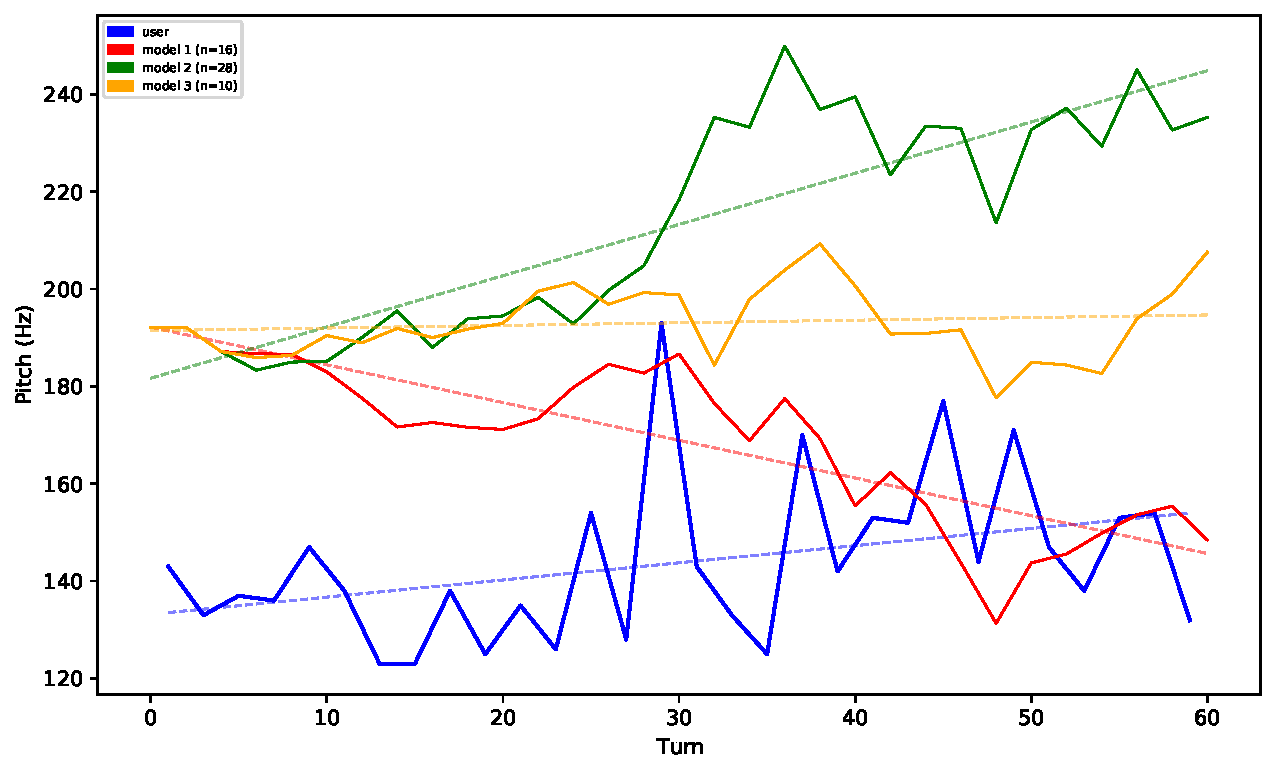
\includegraphics[width=\textwidth]{incr_gen_models}
	\caption[Probabilistic generation of captured accommodation behaviors]
		{Responses of the three models, generated for the same user input (in blue).
	 	 The dashed lines show the linear overall trend of the solid line of the same color.
	 	 Note that these lines should be taken a reference for the general trend and \textbf{not as a representation or estimation of the values}.}
	\label{fig:incr_gen_models}
\end{figure}

This process was used to simulate accommodation changes during a conversation using the three clusters from \cref{fig:k-means_clustering}.
Although the dataset used here is relatively small and is not designed to trigger different behaviors, the natural tendencies of the participants should be, at least to some extent, reflected in this latent representation and be expressed in these simulations.
For each cluster, an n-gram model was created as described in \cref{subsec:word_extraction_and_seq_prob}, based only on the interactions from this cluster.
These models were then used to generate turn-level accommodation response sequences similarly to those in \cref{tab:generated_symbol_sequences}, but longer and with concrete values in addition to their labels.
However, this time the generation was only for the system's side, given a pre-defined input of a human use, simulating a live interaction.
In the example showed here, raw production values from interaction \texttt{20171201B\_Calendar\_02} were used.
The first 30 rounds (60 turns) of three hypothetical conversations for this input were generated, one per model.
N-grams of length ten were used, to take advantage of the larger context available in this longer interaction.
All the models started with the mean value of the system productions in the dataset.
This would be known also in a real-world scenario from the development of the system's \ac{tts} component and hence doesn't break the principle that only data available in a real-time conversation can be used.
%An arbitrary suitable value can be chosen as a starting value as well.
\Cref{fig:incr_gen_models} shows the simulated interactions.
The trend lines show that, by and large, each model behaves differently:
The green line tends towards divergence from the user, the red one inclines to convergence, and the yellow stays roughly the same regardless of the user's productions.
These tendencies intensify once the user starts to show stronger variation around turns 35-40, and subsequently to a lesser extent till the end.
Following these turns, the green line goes more sharply up, the red more sharply down, and the somewhat more neutral yellow starts to wiggle more.
It can be claimed, therefore, that certain core behaviors were captured by the models, and they are sensitive to external input.
This emphasizes the need to look at accommodation as a mutual process occurring in context over time and not as a discretized one-sided phenomenon, even if each speaker has an inert typical behavior.
Noticeably, around turn 50 the red line goes down to \ac{f0} values that might sound untypical for a female speaker (or just overly converging in general).
% female because the data is taken from a female Alexa voice
This is due to the fact that the models here learn some theoretical probabilistic accommodative behavior, but do not have any knowledge about realistic human speech.
Such issues can be easily addressed by applying policies based either on data and expert knowledge, as explained and demonstrated in \cref{subsec:comb_comp_stat_models}.